% arr: add line, change color
\documentclass[tikz,border=10pt]{standalone}

\usepackage{tikz}

\begin{document}

% draw ticks
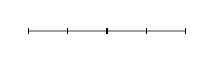
\begin{tikzpicture}
	% If you provide two numbers before the ..., the \foreach statement will use their difference for the stepping:
	\draw[gray!75] (-1,0) -- (1, 0);   % draw line
	\foreach \x in {-1,-0.5,...,1}
		\draw (\x cm,-1pt) -- (\x cm,1pt);
\end{tikzpicture}

\end{document}
